\hei{34题、结合材料回答问题:}

\qquad \kai{华佗是我国东汉名医。一次,府吏倪寻和李延俩人均头痛发热。一同去请华佗诊治,华佗经过仔细的望色、诊脉,开出两付不同的处方。给倪寻开的是泻药,给李延开的是解表发散药。二人不解:我俩患的是同一症状,为何开的药方却不同呢?是不是华佗弄错了?于是,他们向华佗请教。华佗解释道:倪寻的病是由于饮食过多引起的,病在内,应当服泻药,将积滞泻去,病就好了。李延的病是受凉感冒引起的,病在外,应当吃解表药,风寒之邪随汗而去,头痛也就好了。你们病症相似,但病因相异,所以治之宜殊。二人拜服,回家后各自将药熬好服下,很快都痊愈了。}

\qquad \kai{中医是我国宝贵的医学遗产,强调辩证施治。华佗对症下药治头痛发热的故事含蕴丰富的辩证法思想。}

(1)指出其中所涉及的唯物辩证法基本范畴并分析其内涵。(6分)

(2)这个故事对我们理解“具体问题具体分析”有何启示?(4分)

\clearpage

\hei{35题、结合材料回答问题:}

\hei{材料1}

\begin{center}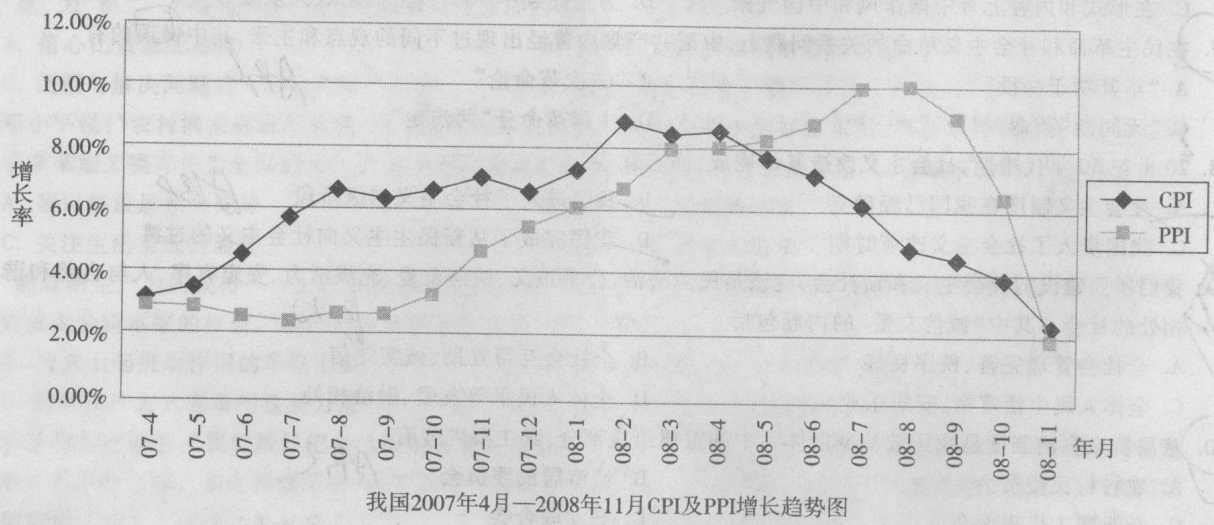
\includegraphics{35.jpg}\end{center}

\begin{center}我国2007年4月-2008年11月CPI及PPI增长趋势图\end{center}

\qquad \kai{注:CPI(消费价格指数)是反映一定时期内城乡居民家庭购买的生活消费品的价格和服务项目价格变动趋势和程度的相对数,一般认为CPI的增幅大于3%时,就存在通货膨胀的压力。PPI(生产价格指数)是衡量工业企业产品价格变动趋势和变动程度的指标。}

\begin{flushright}\kai{资料来源:国家统计局公布数据}\end{flushright}

\hei{材料2}

\qquad \kai{我国经济自2003年进入新一轮上升期,经济增长速度从2003年的10\%一路上涨,2006年突破11\%,并于2007达到11.9\%。然而经济偏快增长也带来一系列影响经济社会可持续发展的重大问题,经济增长有可能由偏快转为过热。2007年12月初召开的中央经济工作会议确定的宏观调控任务是:“防止经济增长由偏快转为过热,防止价格由结构性上涨演变为明显通货膨胀。”}

\qquad \kai{2008年,随着国际经济金融危机的不断加深,国内许多外向型出口企业经营出现困难,出口持续出现下滑势头。上半年经济增长开始放缓,GDP同比增长10.4\%,比去年同期回落1.8\%,上半年居民消费价格水平上涨7.9\%,这表明“防过热”已见效,但物价涨幅较高仍未得到有效控制。2008年7月25日召开的中央政治局会议明确了下半年经济工作的任务:把保持经济平稳较快发展,控制物价过快上涨放在突出的位置,即“一保一控”。财政部等部门宣布自2008年8月1日起提高部分出口商品的退税率,央行8月初调整了商业银行信贷规模,9月16日起又下调了人民币贷款基准利率和中小金融机构人民币存款准备金率,以缓解中小企业融资难、担保难以及流动资金短缺等问题。}

\qquad \kai{2008年前三季度,我国经济增速同比回落了2.3个百分点,经济增长五年多首次低于10\%,随着国际经济金融危机对我国实体经济影响日益显现,国内经济的下行风险逐步加大,中国已经从持续升温转入降温状态。11月9日国务院宣布实行积极的财政政策和适度宽松的货币政策,特别是拉动内需十项新举措的公布。释放出“保增长”的强烈信号,四万亿的投资将对经济产生最直接的拉动。十二月中央经济工作会议进一步明确指出必须把保持经济平稳较快发展作为明年经济工作的首要任务。要着力在保增长上下功夫,把扩大内需作为保增长的根本途径,把加快发展方式转变和结构调整作为保增长的主攻方向。把深化重点领域和关键环节改革,提高对外开放水平作为保增长的强大动力,把改善民生作为保增长的出发点和落脚点。}

\begin{flushright}\kai{资料来源:财政部网站、新浪财经网等}\end{flushright}

问题:

(1)CPI与PPI的走势及其变化反映我国经济运行出现了什么问题?结合材料分析导致这些变化的主要原因。(4分)

(2)结合材料分析我国政府根据国内外经济形势的变化,运用财政政策和货币政策来实施宏观调控。(6分)

\clearpage

\hei{36. 结合材料回答问题:}

\hei{材料1}

\qquad \kai{矛盾是普遍存在的,不过按事物的性质不同,矛盾的性质也就不同。}

\qquad \kai{社会主义社会的矛盾同旧社会的矛盾,例如同资本主义社会的矛盾,是根本不相同的。资本主义社会的矛盾表现为剧烈的对抗和冲突,表现为剧烈的阶级斗争,那种矛盾不可能由资本主义制度本身来解决,而只有社会主义革命才能够加以解决。社会主义社会的矛盾是另一回事,恰恰相反,它不是对抗性的矛盾,它可以经过社会主义制度本身,不断地得到解决。}

\qquad \kai{在社会主义社会中,基本的矛盾仍然是生产关系和生产力之间的矛盾,上层建筑和经济基础之间的矛盾。不过社会主义社会的这些矛盾,同旧社会的生产关系和生产力的矛盾、上层建筑和经济基础的矛盾,具有根本不同的性质和情况罢了。}

\qquad \kai{社会主义生产关系已经建立起来,它是和生产力的发展相适应的;但是,它又还很不完善,这些不完善的方面和生产力的发展又是相矛盾的。除了生产关系和生产力发展的这种又相适应又相矛盾的情况以外,还有上层建筑和经济基础的又相适应又相矛盾的情况。}

\begin{flushright}\kai{摘自毛泽东《正确处理人民内部矛盾的问题》(1957年2月27日)}\end{flushright}

\hei{材料2}

\qquad \kai{社会主义社会的基本矛盾和目前时期的主要矛盾。关于基本矛盾,我想现在还是按照毛泽东同志在《关于正确处理人民内部矛盾的问题》一文中的提法比较好。毛泽东同志说:“在社会主义社会中,基本的矛盾仍然是生产关系和生产力之间的矛盾,上层建筑和经济基础之间的矛盾。”他在这里说了很长的一段话,现在不重复。当然,指出这些基本矛盾,并不就完全解决了问题,还需要就此作深入的具体的研究。但是从二十多年的实践看来,这个提法比其他的一些提法妥当。至于什么是目前时期的主要矛盾,也就是目前时期全党和全国人民所必须解决的主要问题或中心任务,由于三中全会决定把工作重点转移到社会主义现代化建设方面来,实际上已经解决了。我们的生产力发展水平很低,远远不能满足人民和国家的需要,这就是我们目前时期的主要矛盾,解决这个主要矛盾就是我们的中心任务。}

\begin{flushright}\kai{摘自邓小平《坚持四项基本原则》(1979年3月30日)}\end{flushright}

结合材料回答问题:

(1)毛泽东提出社会主义社会基本矛盾的历史背景及这一理论的重大意义(6分)

(2)邓小平关于社会主义基本矛盾“深入的具体的研究”所取得的理论成果主要有哪些?(4分)

\clearpage

\hei{37. 结合材料回答问题:}

\hei{材料1}

\qquad \kai{从1978年到2007年,我国国内生产总值由3645亿元增长到24.95万亿元,年均实际增长9.8\%,是同期世界经济年均增长率的3倍多,我国经济总量上升为世界第四。}

\qquad \kai{从1978年到2007年,我国进出口总额从206亿美元提高到21737亿美元,跃居世界第三位。}

\qquad \kai{外汇储备从长期没有达到10亿美元,提高到2007年的1.5万亿美元左右,成为世界上拥有外汇储备最多的国家。}

\qquad \kai{从1978年到2007年,全国城镇居民人均可支配收入由343元增加到13786元,实际增长6.5倍。农民人均纯收入则由134元增加到4140元,实际增长6.3倍;农村贫困人口从2.5亿减少到1400多万。}

\begin{flushright}\kai{摘自胡锦涛在纪念党的十一届三中全会30周年大会上的讲话}\end{flushright}

\hei{材料2}

\qquad \kai{改革开放以来我们取得一切的成绩和进步的根本原因,归结起来就是:开辟了中国特色社会主义道路,形成了中国特色社会主义理论体系。高举中国特色社会主义伟大旗帜,最根本的就是要坚持中国特色社会主义道路和中国特色社会主义理论体系。}

\begin{flushright}\kai{摘自胡锦涛在中国共产党的第十七次全国代表大会上的报告}\end{flushright}

(1)改革开放30年来,我国经济体制进行了哪些主要的改革创新才带来了上述变化?(5分)

(2)简述中国特色社会主义理论体系的组成部分及其所要回答的基本问题。(5分)

\clearpage

\hei{38题、}本题为选做题,请在Ⅰ、Ⅱ两道试题中选取其中一道作答,若两题都回答,只按第Ⅰ道试题的成绩记入总分。

\vspace{6pt}

\hei{选做题Ⅰ}

\hei{材料1}

\qquad \kai{如果美国不援助欧洲,它们在经济、政治和社会关系各方面都将有窒息之虞,美国这次“援欧”不同于以往,不是向个别国家提供零星援助,而是向联合的欧洲提供援助。我们的政策不是反对任何国家、任何主义,而是反对饥饿、贫穷、悲惨、混乱。我们的任务是唤起合理经济的再生,促进政治社会的结构容纳自由制度存在。任何企图阻碍别国复兴的政府,都不会得到我们的帮助。任何政府、党派为图政治私利或其他打算,不惜延续人类痛苦的,必会遭到美国的反对。}

\begin{flushright}\kai{摘编自马歇尔在哈佛大学的演讲(1947年6月5日)}\end{flushright}

\hei{材料2}

\qquad \kai{2002年1月,美国国务卿鲍威尔访问尼泊尔,主要讨论反恐合作问题,此后,美国每年向尼泊尔提供4000万美元的“经济援助”。2003年11月3日,美国国会批准了向伊拉克和阿富汗提供875亿美元的军事行动及重建援助的拨款法案。西方把这些经济援助和重建计划称为“新马歇尔计划”。}

\qquad \kai{伊拉克已探明拥有1100亿桶的石油储藏,远景储量达2200亿桶,开采成本每桶仅3-4美元。2003年12月,美国国防部公布了伊拉克重建项目中总价值达186亿美元的26个重大工程合同,同时以维护美国的“基本安全利益”为由,决定剥夺包括德国、法国、俄罗斯、加拿大等在内的100多个曾经反对美国发动伊拉克战争以及拒绝向伊拉克派兵的国家参与上述合同的竞标资格。首批约9亿美元的伊拉克重建合同均在暗盘交易下完成,中标的是清一色的美国公司,而这些公司无不与美国政府有着紧密的联系。}

\begin{flushright}\kai{摘编自人民网}\end{flushright}

\hei{材料3}

\qquad \kai{法国前情报员达尼埃尔·雷米在其所著《谁欲杀死法兰西》一书中认为,美国已经发动了一场看不见的“经济战争”,旨在征服欧洲。1995年至1999年间,美国每年立案的反倾销和反补贴调查中,有1/4是针对欧盟的。}

\qquad \kai{德国和法国不赞成美国对伊拉克动武,惹怒了美国,美前国防部长拉姆斯菲尔德抨击两国“有问题”;时任美国总统国家安全事务助理的赖斯,把包括法国与德国在内的反战政府比作是“二战”前法国对纳粹德国的“姑息主义”,引起德、法等国不满,美前国务卿基辛格认为,在伊拉克问题上的分歧,已经在大西洋联盟中产生了自它50年前成立以来最为严重的危机。}

\begin{flushright}\kai{摘编自中国网}\end{flushright}

结合材料回答问题:

(1)结合材料一、二比较“马歇尔计划”和“新马歇尔计划”的异同。(5分)

(2)结合材料一、三,剖析近些年来美、欧在处理国际事务中,显现的分歧和原因。(5分)

\vspace{6pt}

\hei{选做题Ⅱ、}阅读下列材料:

\hei{材料1}

\qquad \kai{近年来,越来越多的国家和国际知名人士开始热议“中国贡献”,关于中国在地区和全球事物中发挥重要建设性作用的话语频现于国际社会。}

\qquad \kai{阿拉伯国家联盟负责政治事务的副秘书长本·哈拉2007年4月14日,在会见中国驻阿盟全权代表吴恩科大使时说,阿盟高度赞誉中国在解决苏丹达尔富尔问题上发挥的积极作用,中国关于解决该问题的立场是公正、积极和平衡的,所发挥的作用是建设性的,有深远的影响力。第一届东盟秘书长、泰国前外长素林2008年1月7日在回答记者提问时表示,中国积极支持东盟组织的发展,同时积极参与解决本地区以及国际事务,中国为提升整个东亚地区自信力做出了很大贡献,中国在东亚地区所做的贡献,对地区发展给予的大力支持以及所发挥的建设性作用,让东盟信服。}

\begin{flushright}\kai{摘自《理论热点面对面·2008》}\end{flushright}

\hei{材料2}

\qquad \kai{改革开放以来,中国政府和人民高举和平、发展、合作的旗帜,加强与世界各国的联系和交往,积极参与国际事务,在谋求自身发展的同时,以实际行动在世界上发挥着重要建设性作用。中国认真落实联合国千年发展目标,迄今已向120多个国家和区域组织提供了2000多个援助项目,已累计对49个不发达国家免除到期政府债务374笔。中国已签署了300多个国际公约,参加了130多个国际组织,并在军备控制、贸易投资等国际机制中扮演重要角色。有了中国的参与,许多国际热点问题呈现出积极的变化态势。迄今为止,中国共参与了22项联合国维和行动,累计派出维和人员上万人次,现正在执行维和任务的有1900多人。中国自1990年首次参加联合国维和行动以来,累计新建、修复道路7300多公里,桥梁200多座,排除地雷及各类未爆炸物7600多枚,运送人员12万多人次、物资26万多吨,接诊病人3.6万多人次,先后有3名军官和5名士兵在执行维和任务中牺牲。}

\begin{flushright}\kai{摘自《理论热点面对面·2008》}\end{flushright}

结合材料回答问题:

(1)中国积极参与国际事务所发挥的“建设性的、有深远的影响力”的作用表现在哪些方面?(6分)

(2)中国在当今国际事务中能够做出“中国贡献”的原因何在?(4分)
